\documentclass[10pt, a4paper]{article}
\usepackage[a4paper,outer=1.5cm,inner=1.5cm,top=1.75cm,bottom=1.5cm]{geometry}

\twocolumn
\usepackage{graphicx}
\usepackage{karnaugh-map}
\usepackage{tabularx}
\usepackage{hyperref}
\usepackage[utf8]{inputenc}
\usepackage{amsmath}
\usepackage{physics}
\usepackage{amssymb}

\begin{document}
\title{Line Assignment}
\author{Name:A.Gowri Priya\and Email :  \url{gowripriyaappayyagari@gmail.com}}
%\{ Wireless Communication (FWC)}
\date{}
\maketitle


  \section{Problem}
In  $\Delta$  ABC and  $\Delta$ DEF, AB = DE, AB $\parallel$ DE, BC = EF
and BC $\parallel$ EF. Vertices A, B and C are joined to
vertices D, E and F respectively (see Figure).\\
Show that\\
(i) quadrilateral ABED is a parallelogram\\
(ii) quadrilateral BEFC is a parallelogram\\
(iii) AD $\parallel$ CF and AD = CF\\
(iv) quadrilateral ACFD is a parallelogram\\
(v) AC = DF\\
(vi)$\Delta ABC \cong \Delta$  DEF.\\
\begin{figure}[h]
\centering
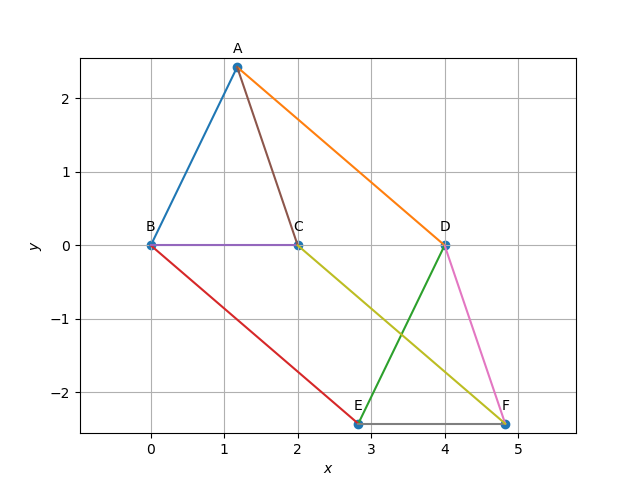
\includegraphics[scale=0.5]{fig.png} 
\caption{Given Figure}
\end{figure}

\section{Solution}
\begin{center}
The input parameters for this construction are
\begin{tabular}{|c|c|}
	\hline
	\textbf{Symbol}&\textbf{Value}\\
	\hline
	r1&2\\
	\hline
	r2&3\\
	\hline
	$\theta$&$\frac{\pi}{2.5}$\\
	\hline
\end{tabular}
\boldmath
$${A}=\begin{pmatrix} r1\cos\theta\\ r2\sin\theta\ \end{pmatrix}$$
$${B}=\begin{pmatrix} 0\\ 0\ \end{pmatrix}$$
$${D}=\begin{pmatrix} 4\\ 0\ \end{pmatrix}$$
$${C}={{B}+{D}}/2$$
$${E}={{B}+{D}-{A}}$$
$${F}={{E}+{C}-{B}}$$
\unboldmath
\end{center}
\textbf{Direction vectors}

The Direction vectors are\\
$\boldsymbol {m_1 = A - B }$\\
$\boldsymbol {m_2 = B - C} $\\
$\boldsymbol {m_3 = A - C} $\\
$\boldsymbol {m_4 = D - E} $\\
$\boldsymbol {m_5 = E - F} $\\
$\boldsymbol {m_6 = D - F} $\\
$\boldsymbol {m_7 = A - D} $\\
$\boldsymbol {m_8 = C - F} $\\\\
\textbf{To proove\\\\ i.Quadrilateral ABED is a parallelogram}\\\\
	Given that 
	AB = DE and AB $\parallel$ DE \\\\
	Directional vectors $\boldsymbol{m_1}$=$\boldsymbol{m_4}$\\\\
i.e $\boldsymbol{{A}-{B}}$ =$\boldsymbol{{D}-{E}}$\\\\
	$\therefore$ Quadrilateral ABED is a parallelogram.\\\\
\textbf{ii.Quadrilateral BEFC is a parallelogram}\\\\
	Given that BC=EF and BC $\parallel$ EF \\\\
	Directional vectors $\boldsymbol{m_2}$=$\boldsymbol{m_5}$\\\\
i.e $\boldsymbol{{B}-{C}}$ =$\boldsymbol{{E}-{F}}$\\\\
	$\therefore$ Quadrilateral BEFC is a parallelogram.\\\\
\textbf{iii.AD$\parallel$CF and AD=CF}\\\\
Directional vectors $\boldsymbol{m_7}$=$\boldsymbol{m_8}$\\\\
i.e $\boldsymbol{{A}-{D}}$ =$\boldsymbol{{C}-{F}} $\\\\	Since the directional vectors AD and CF are same,AD is parallel to CF.\\\\
	$\therefore$ AD$\parallel$CF and AD=CF \\\\
\textbf{iv.Quadrilateral ACFD is a parallelogram}\\\\
Directional vectors $\boldsymbol{m_3}$=$\boldsymbol{m_6}$\\\\
i.e $\boldsymbol{{A}-{C}}$ =$\boldsymbol{{D}-{F}}$\\\\
   $\therefore$ AC$\parallel$DF and AC=DF \\\\
	 $\therefore$ACFD is a parallelogram.\\\\
\textbf{v.AC=DF}\\\\
 Directional vectors $\boldsymbol{m_3}$=$\boldsymbol{m_6}$\\\\
i.e $\boldsymbol{{A}-{C}}$ =$\boldsymbol{{D}-{F}}$\\\\
	$\therefore$ AC=DF\\\\
\textbf{vi.$\Delta $ABC $\cong$ $\Delta$ DEF}  \\\\
$\boldsymbol{\norm{A-B}}$ =$\boldsymbol{\norm{D-E}}$ and $\boldsymbol{\norm{B-C}}$ =  $\boldsymbol{\norm{E-F}}$ and $\boldsymbol{\norm{A-C}}$ =  $\boldsymbol{\norm{D-F}}$\\\\
$\therefore$ By SSS Rule $\Delta ABC \cong \Delta DEF$\\\\

\section{Execution}
*Verify the above proofs in the following code.\\
\framebox{
\url{https://github.com/gowripriya-2002/FWC/blob/main/Matrix/line_assignment/code/line.py}}	
\bibliographystyle{ieeetr}
\end{document}
